Энэ бүлэгт
\section{Функциональ загвар}
МУИС-ийн Дипломын ажлын удирдлагын системийн үндсэн бизнес процессуудыг тодорхойлсон. Зураг \ref{fig:teacher}-т  сэдэв дэвшүүлэх процесс, зураг \ref{fig:student}-т оюутан сэдэв дэвшүүлэх процесс, зураг \ref{fig:topic}-т БСА-ын сонгох процесс, зураг \ref{fig:plan}-т БСА-ын үечилсэн төлөвлөгөөг тэнхимээр батлуулах процесс, \ref{fig:perform}-т БСА гүйцэтгэх, тайлан хураалгах процесс, \ref{fig:evaluate}-т БСА-ыг хамгаалах, дүгнэх процессыг харуулав.

\begin{figure}[H]
  \centering
  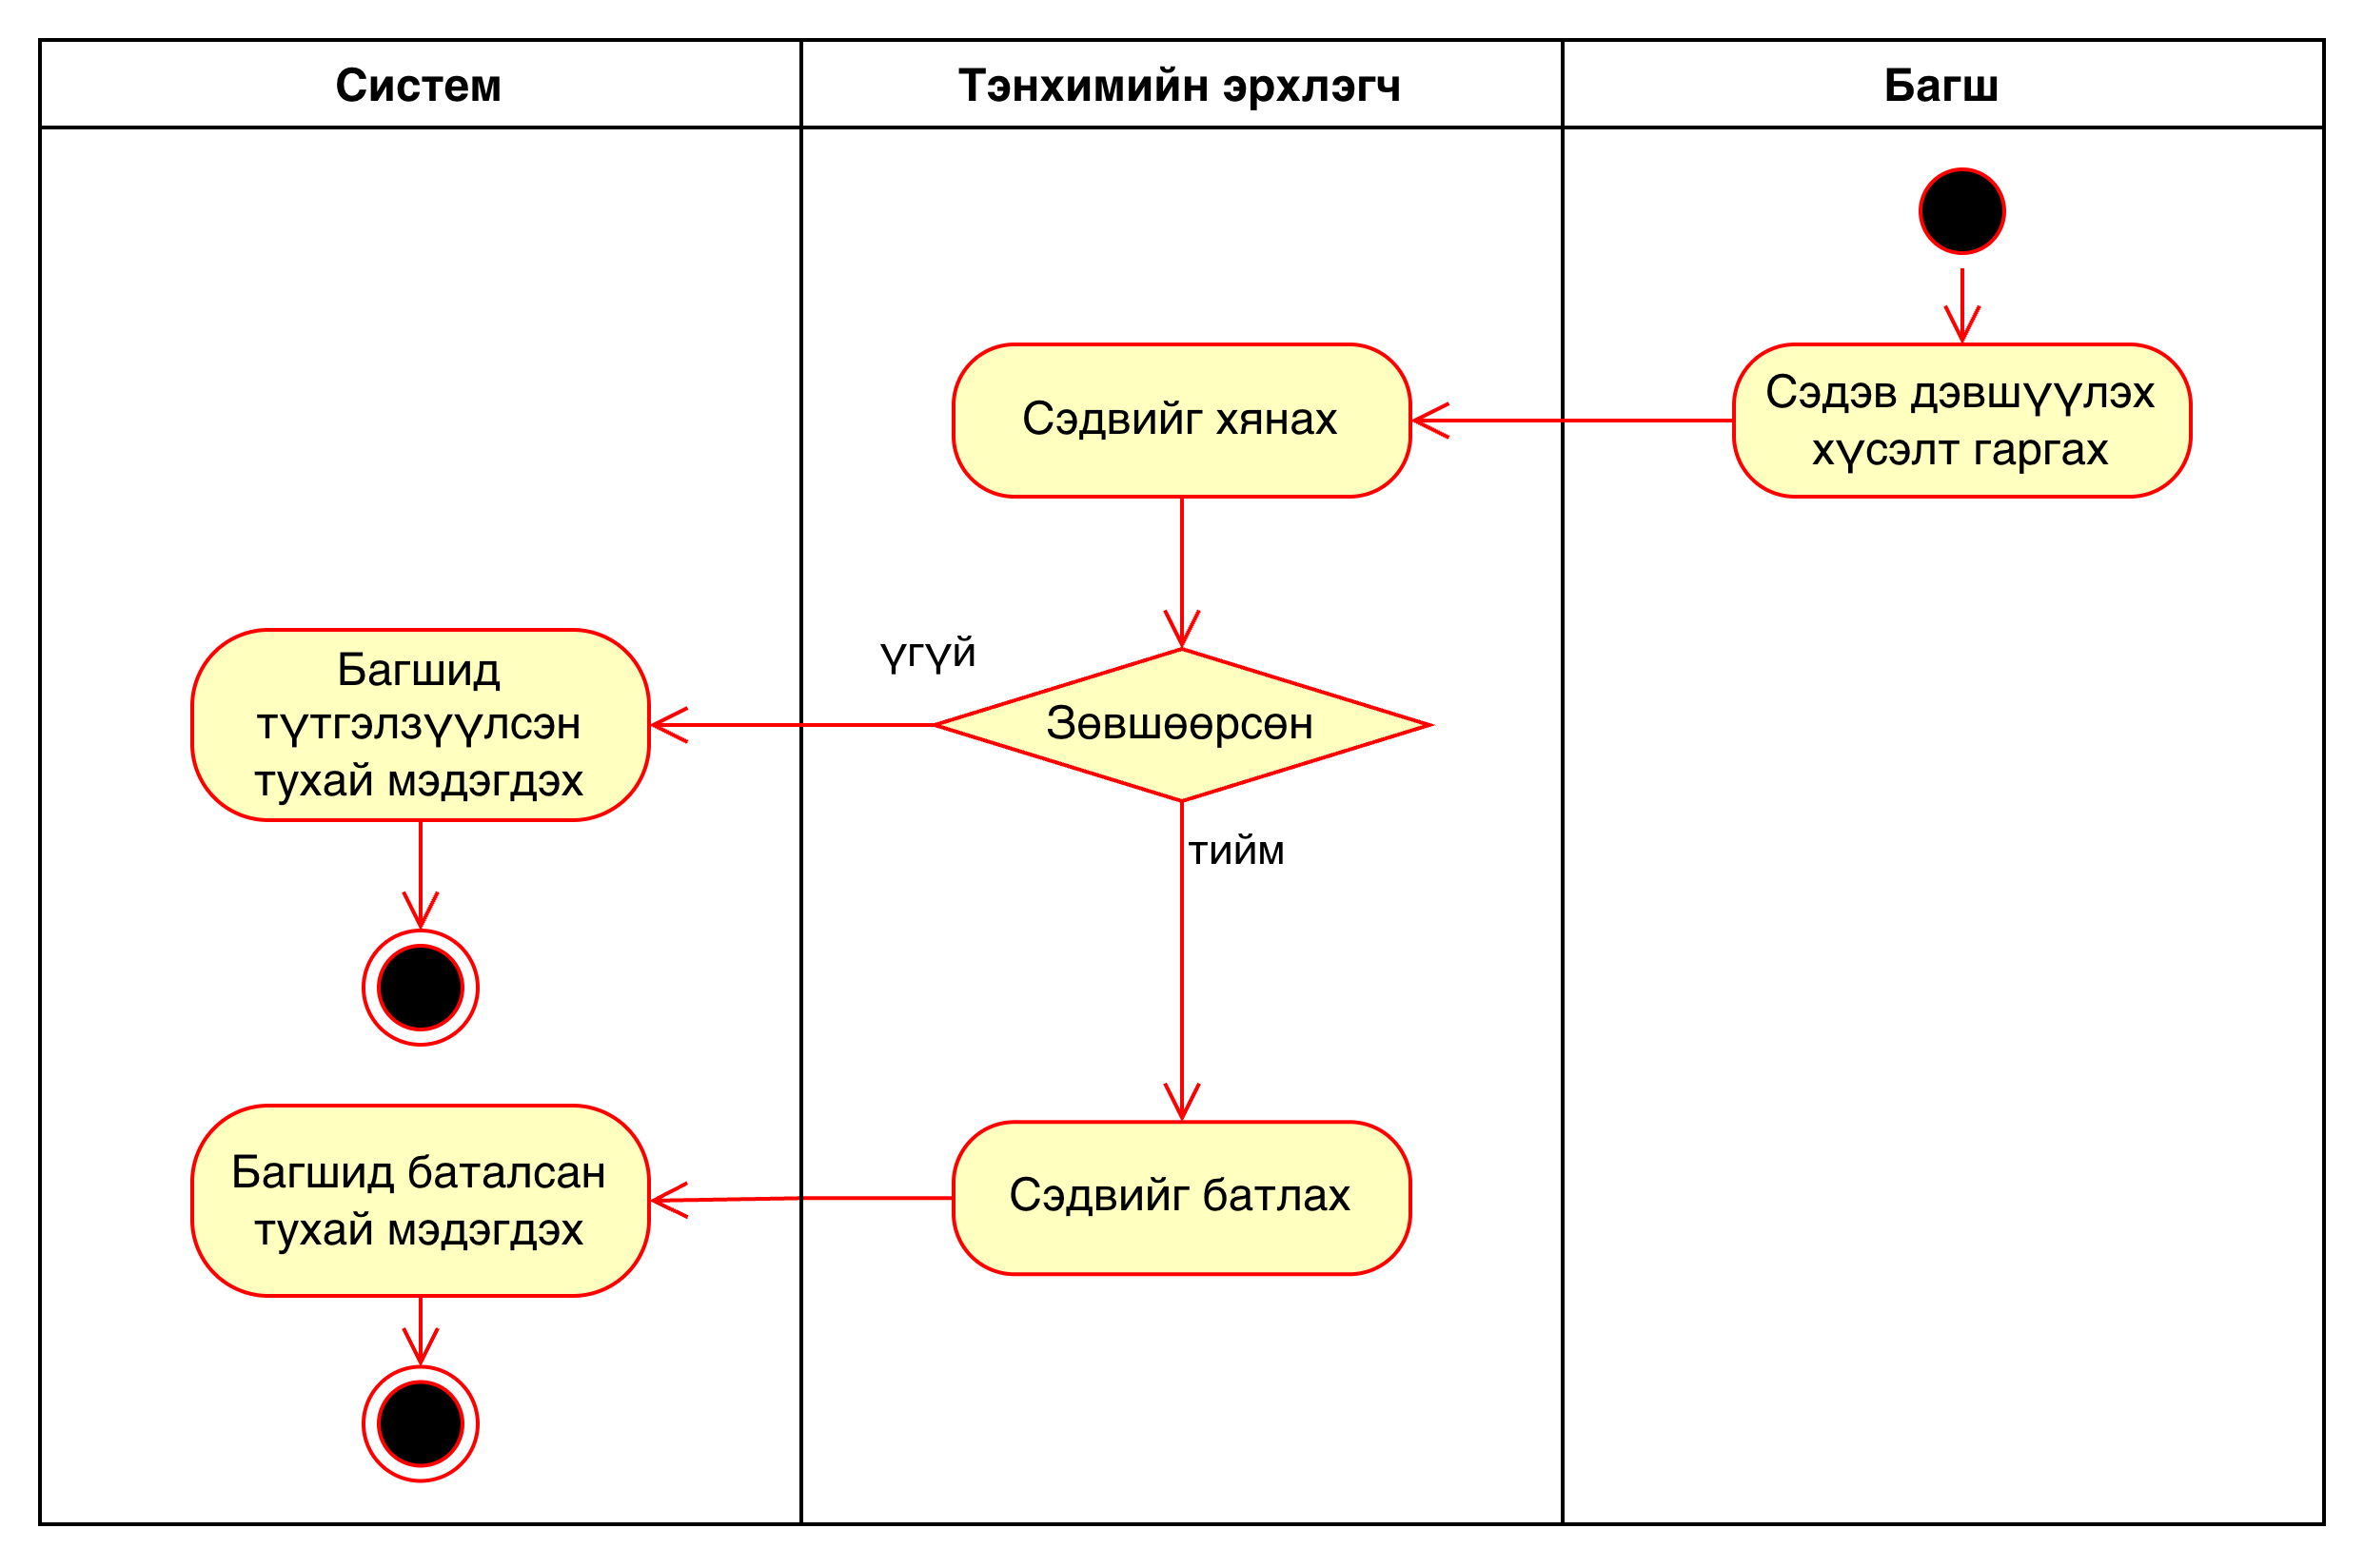
\includegraphics[width=12cm]{images/teacher.png}
  \caption{БСА-ын сэдэв дэвшүүлэх процесс}
  \label{fig:teacher}
\end{figure}

\begin{figure}[H]
  \centering
  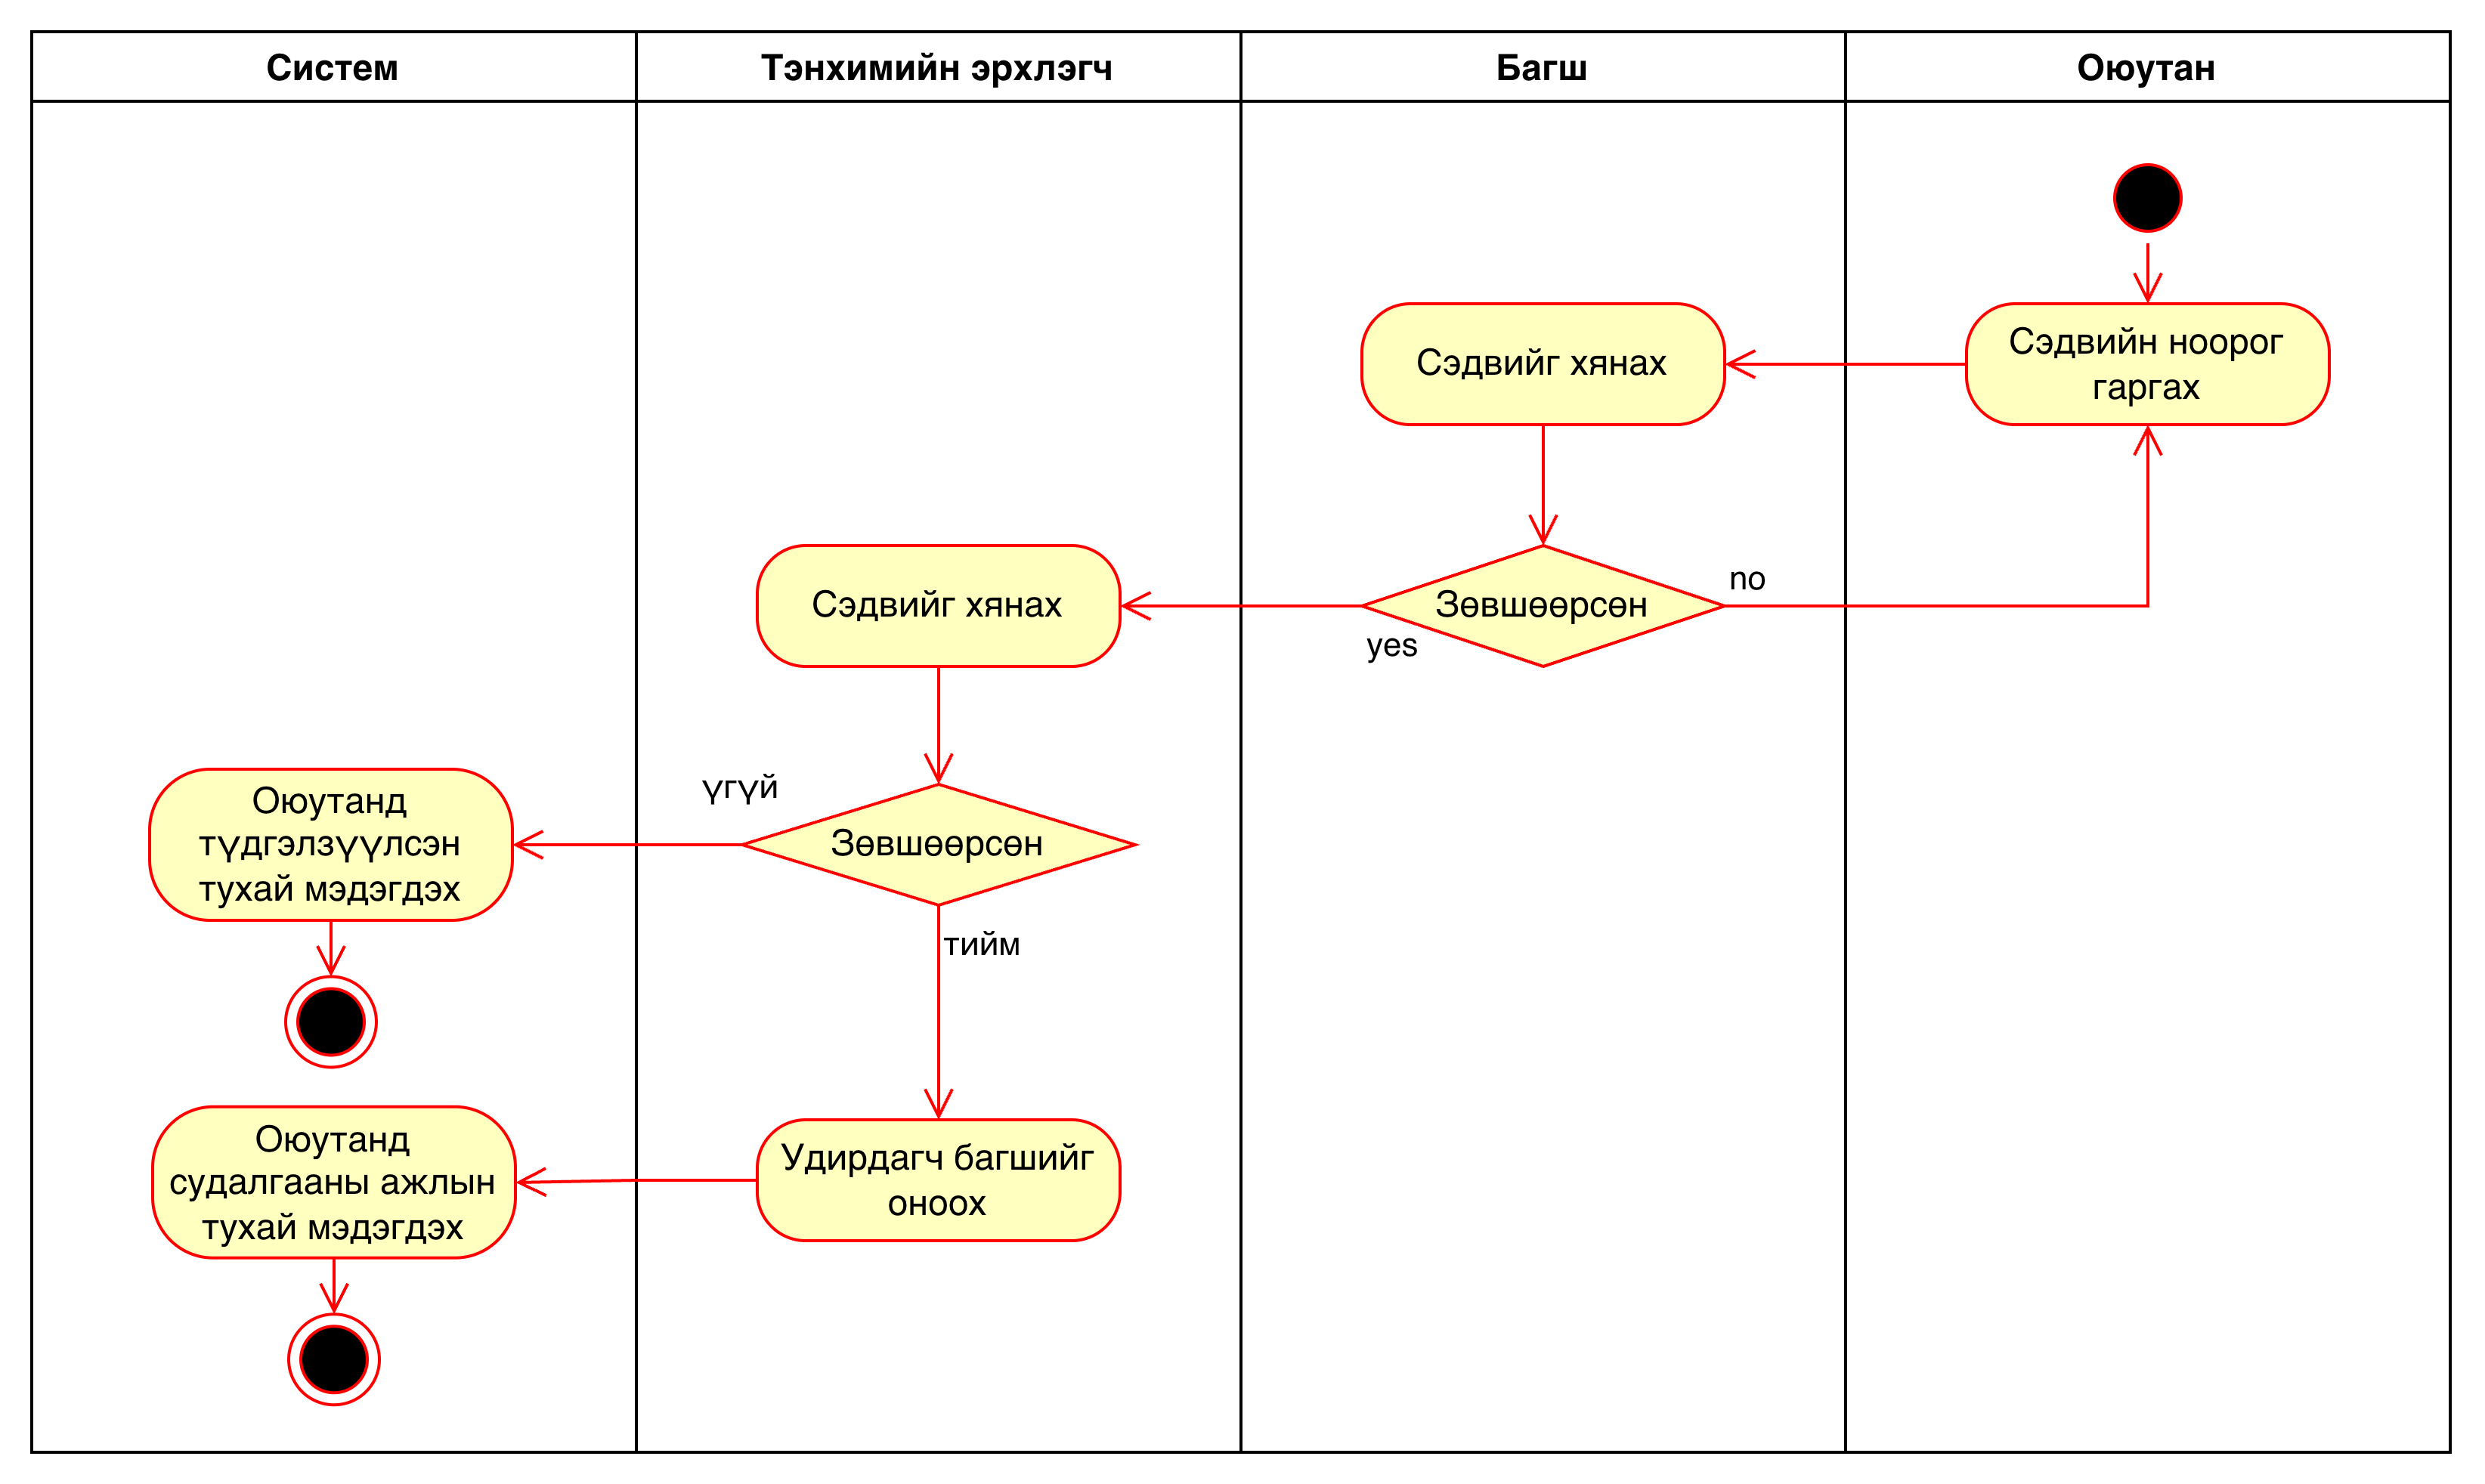
\includegraphics[width=16cm]{images/student.png}
  \caption{БСА-ын сэдэв дэвшүүлэх процессын өргөтгөл}
  \label{fig:student}
\end{figure}

\begin{figure}[H]
  \centering
  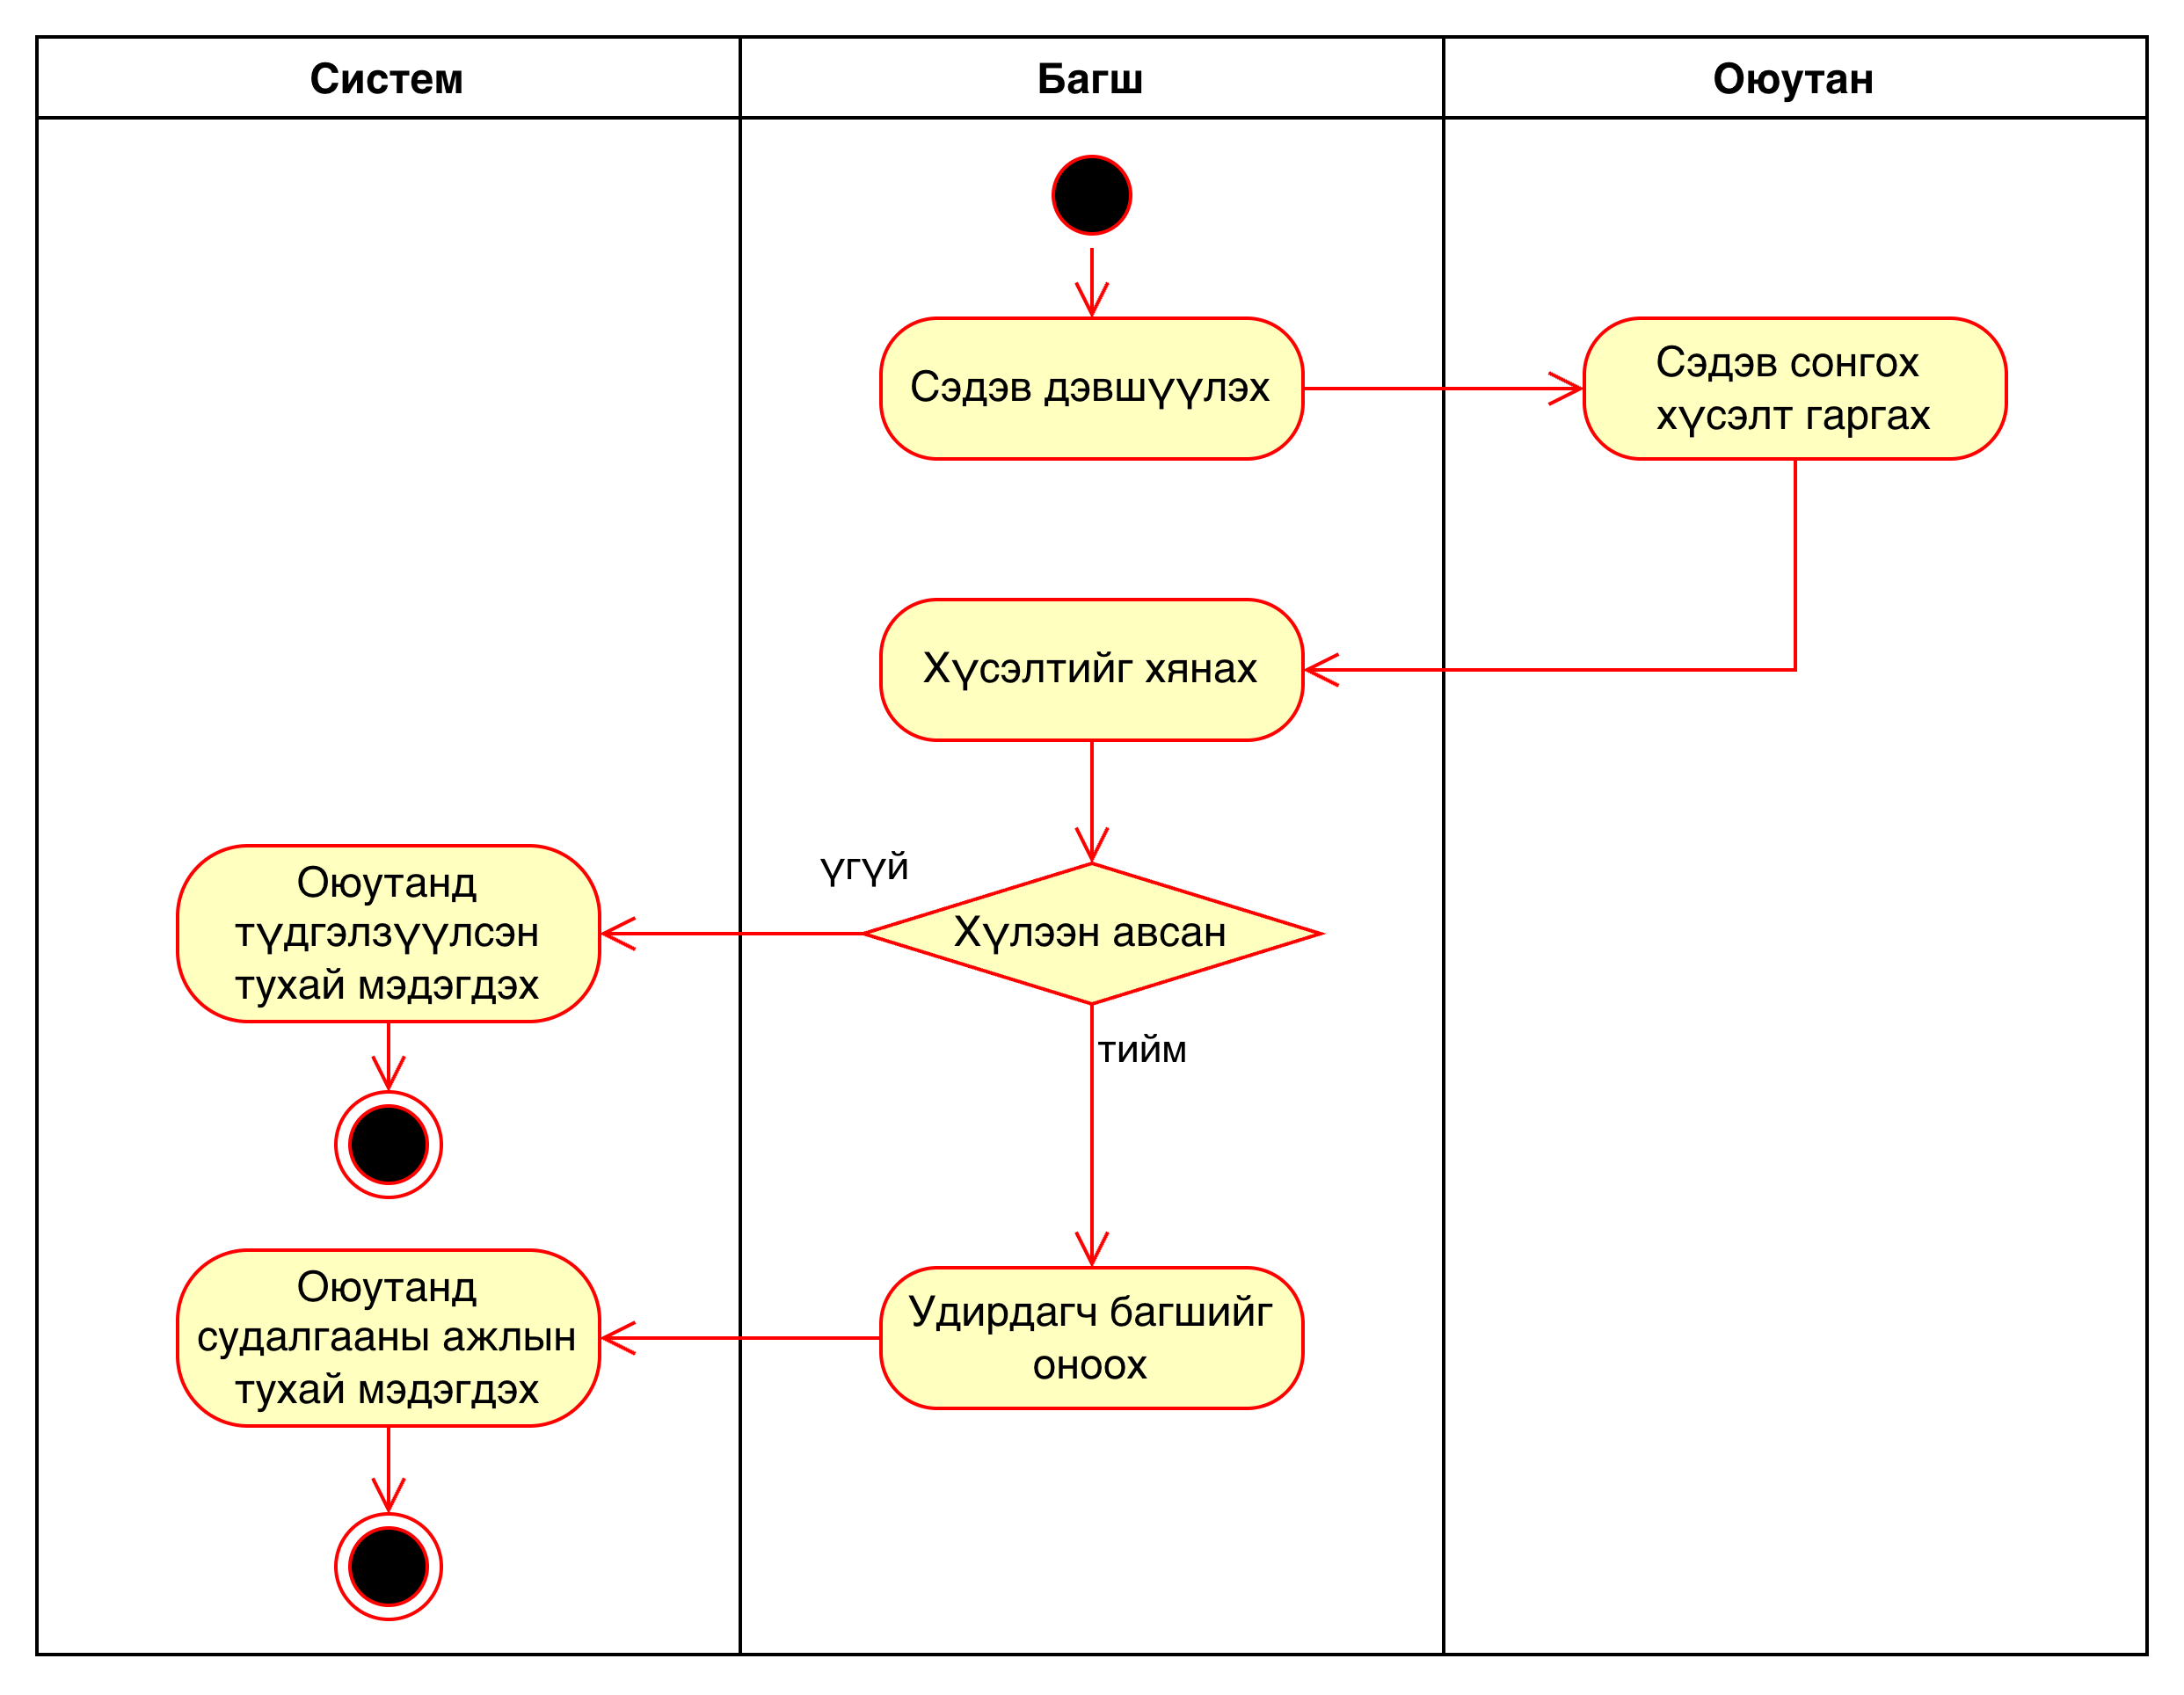
\includegraphics[width=12cm]{images/topic.png}
  \caption{БСА-ын сэдэв сонгох процесс}
  \label{fig:topic}
\end{figure}

\begin{figure}[H]
  \centering
  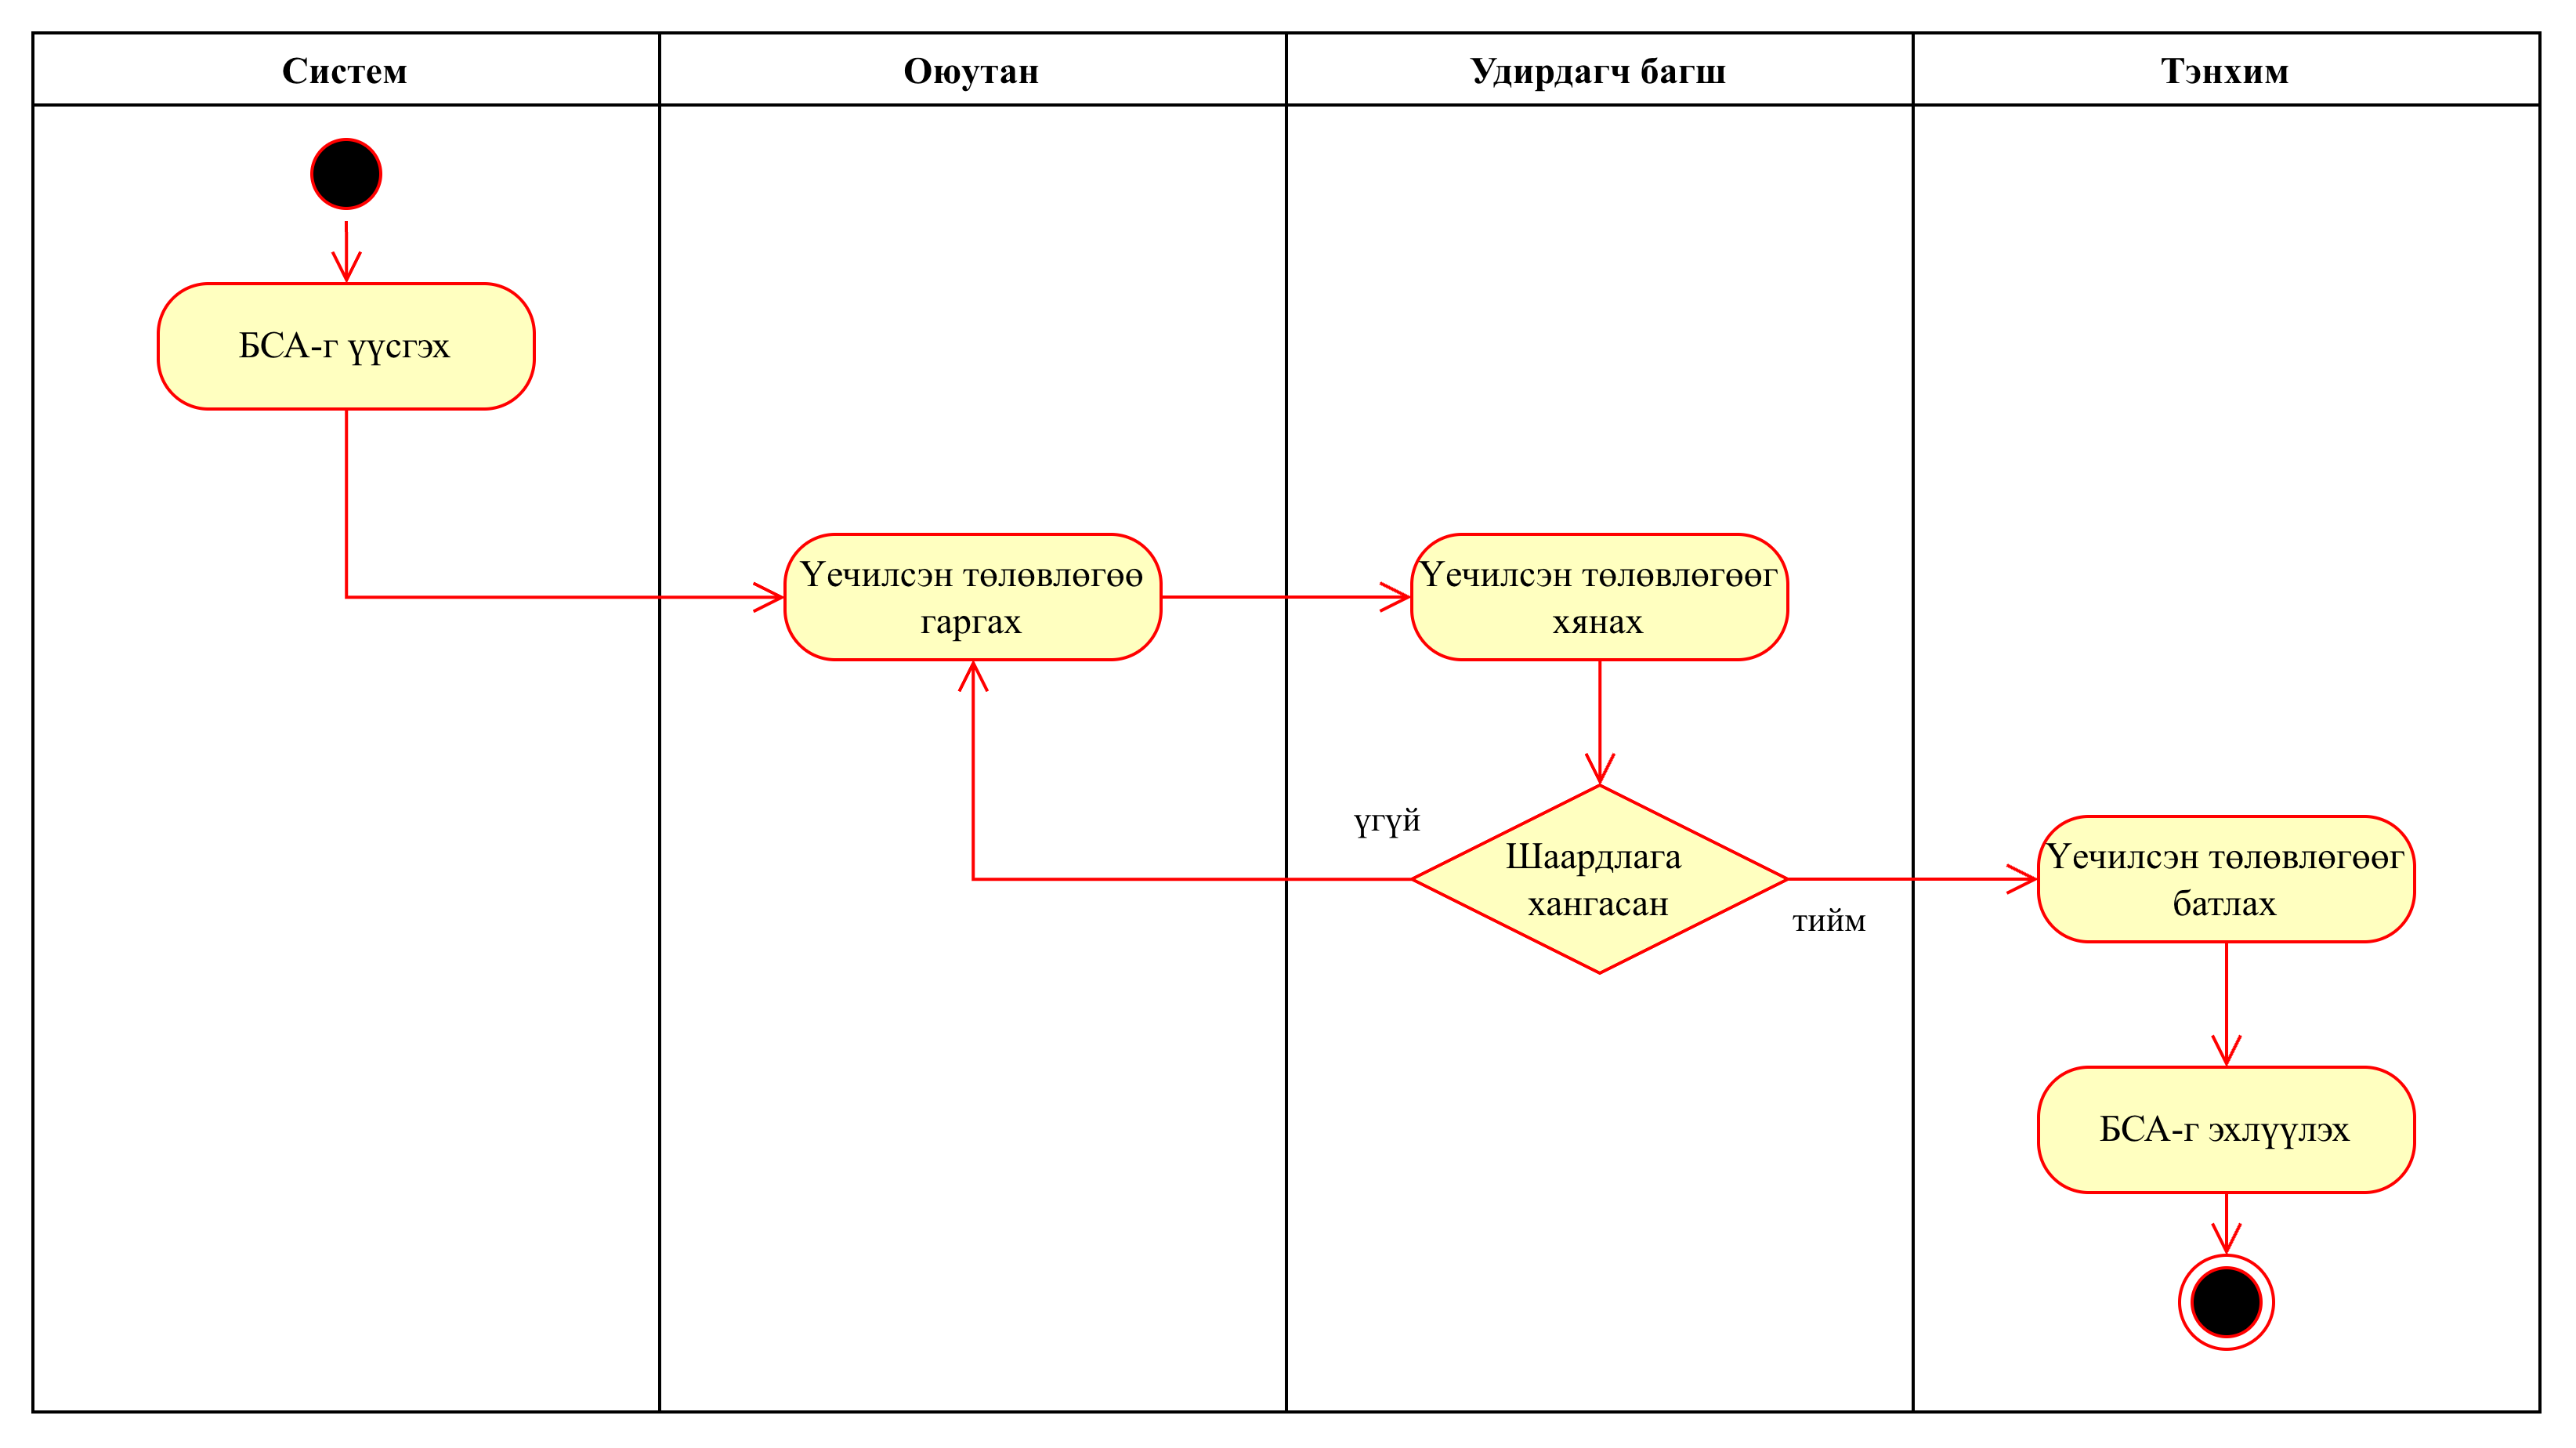
\includegraphics[width=16cm]{images/plan.png}
  \caption{БСА-ын үечилсэн төлөвлөгөөг тэнхимээр батлуулах процесс}
  \label{fig:plan}
\end{figure}

\begin{figure}[H]
  \centering
  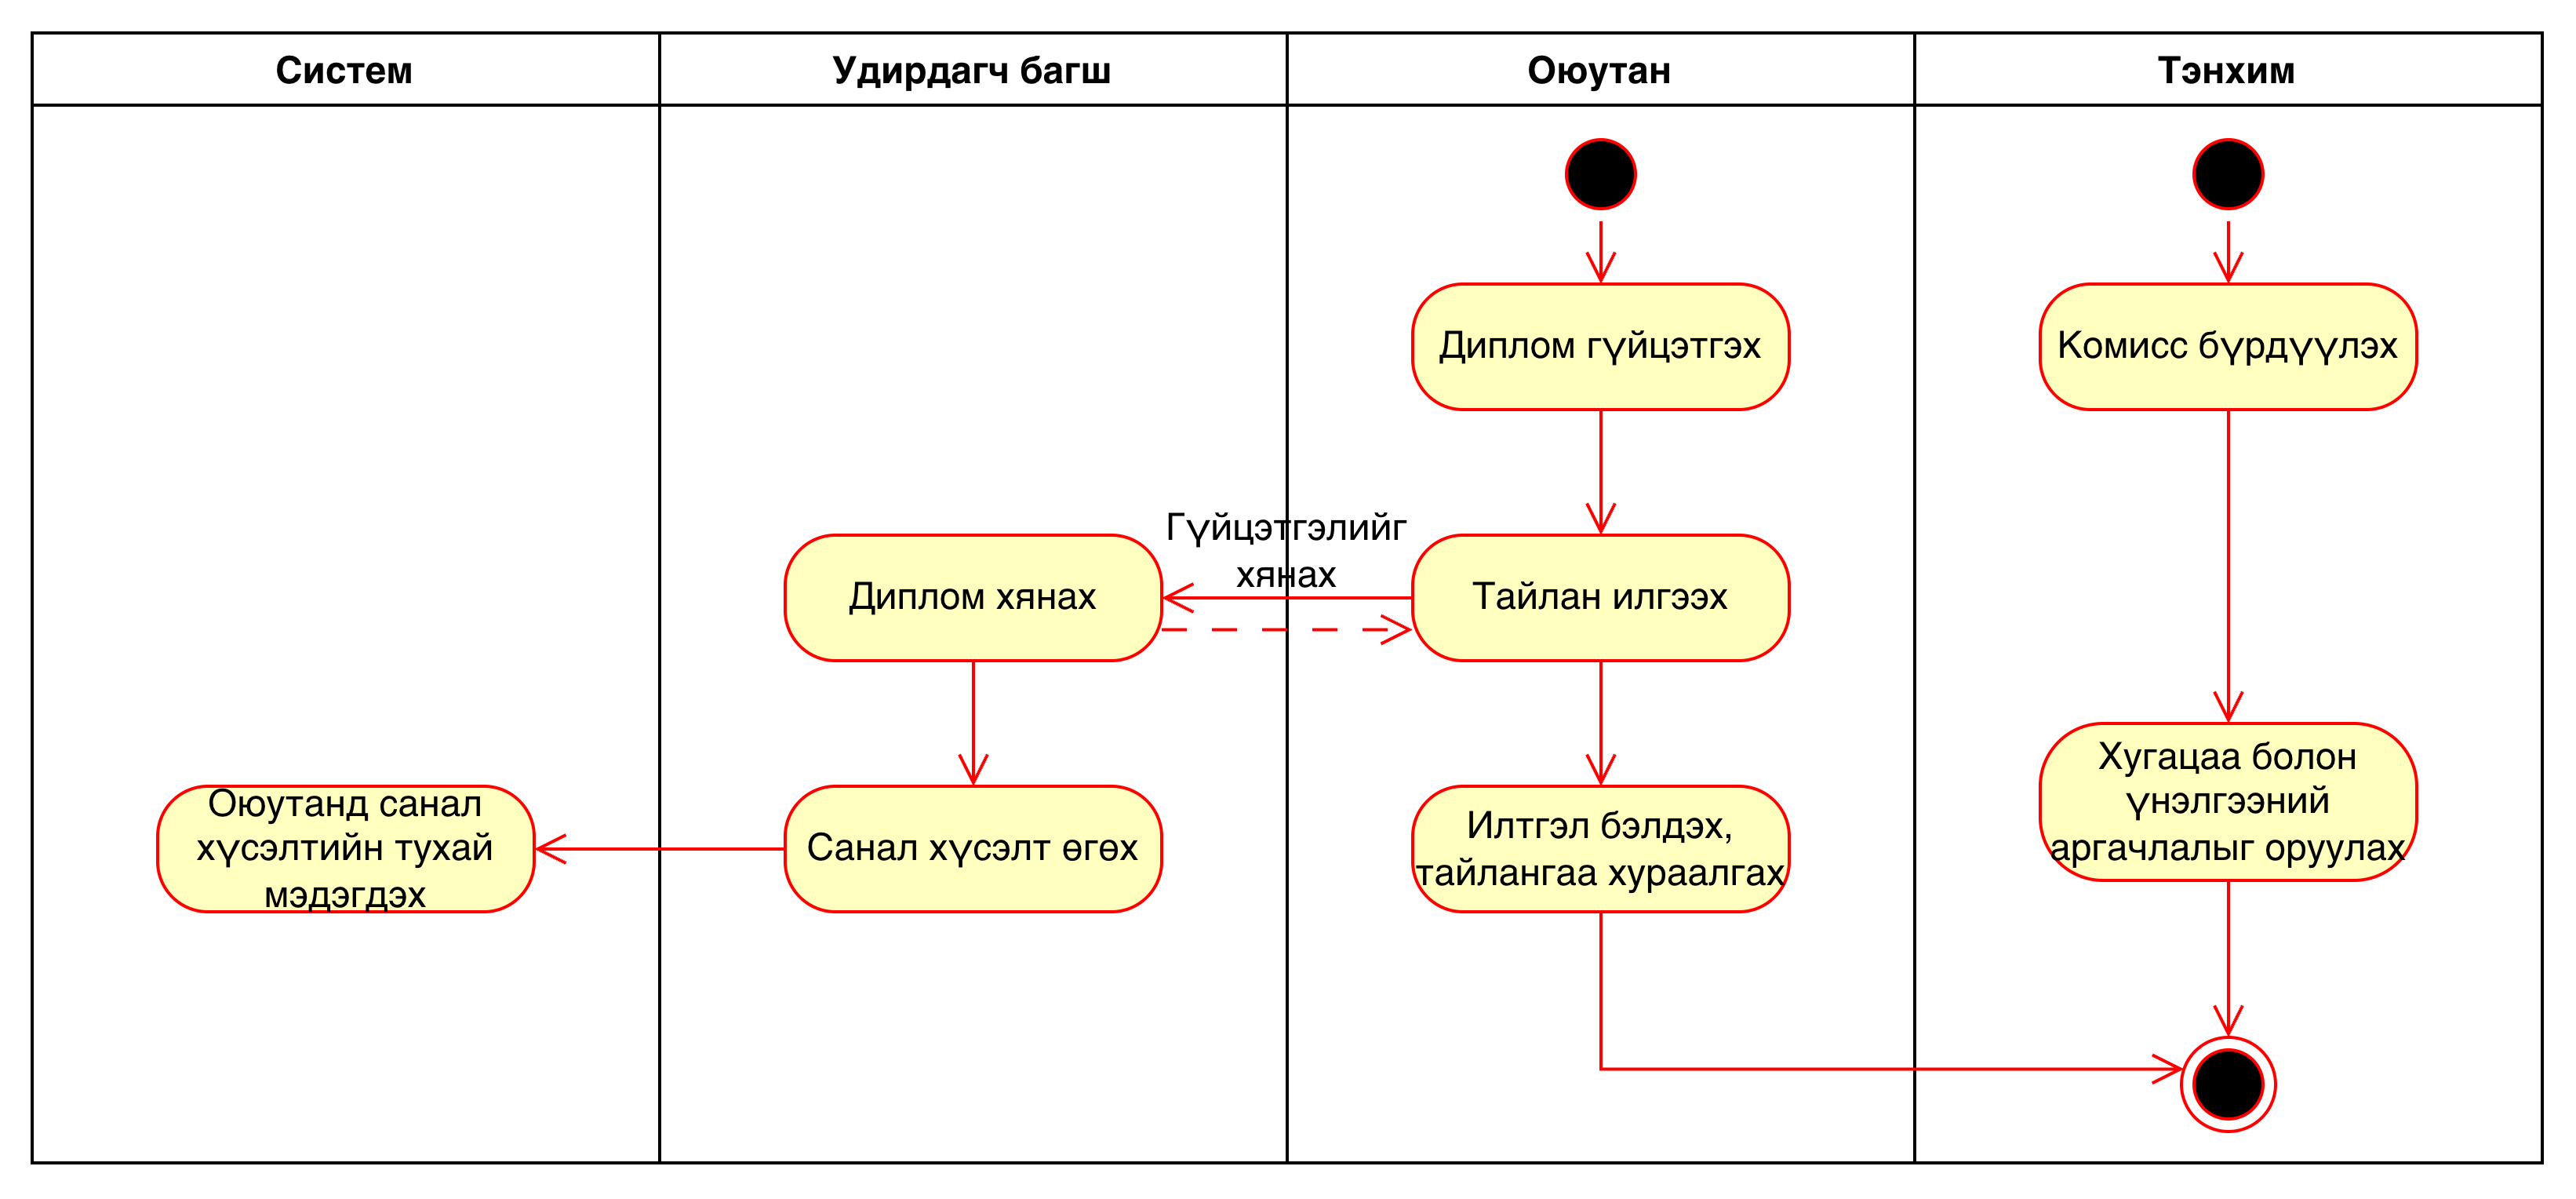
\includegraphics[width=16cm]{images/perform.png}
  \caption{БСА гүйцэтгэх, тайлан хураалгах процесс}
  \label{fig:perform}
\end{figure}

\begin{figure}[H]
  \centering
  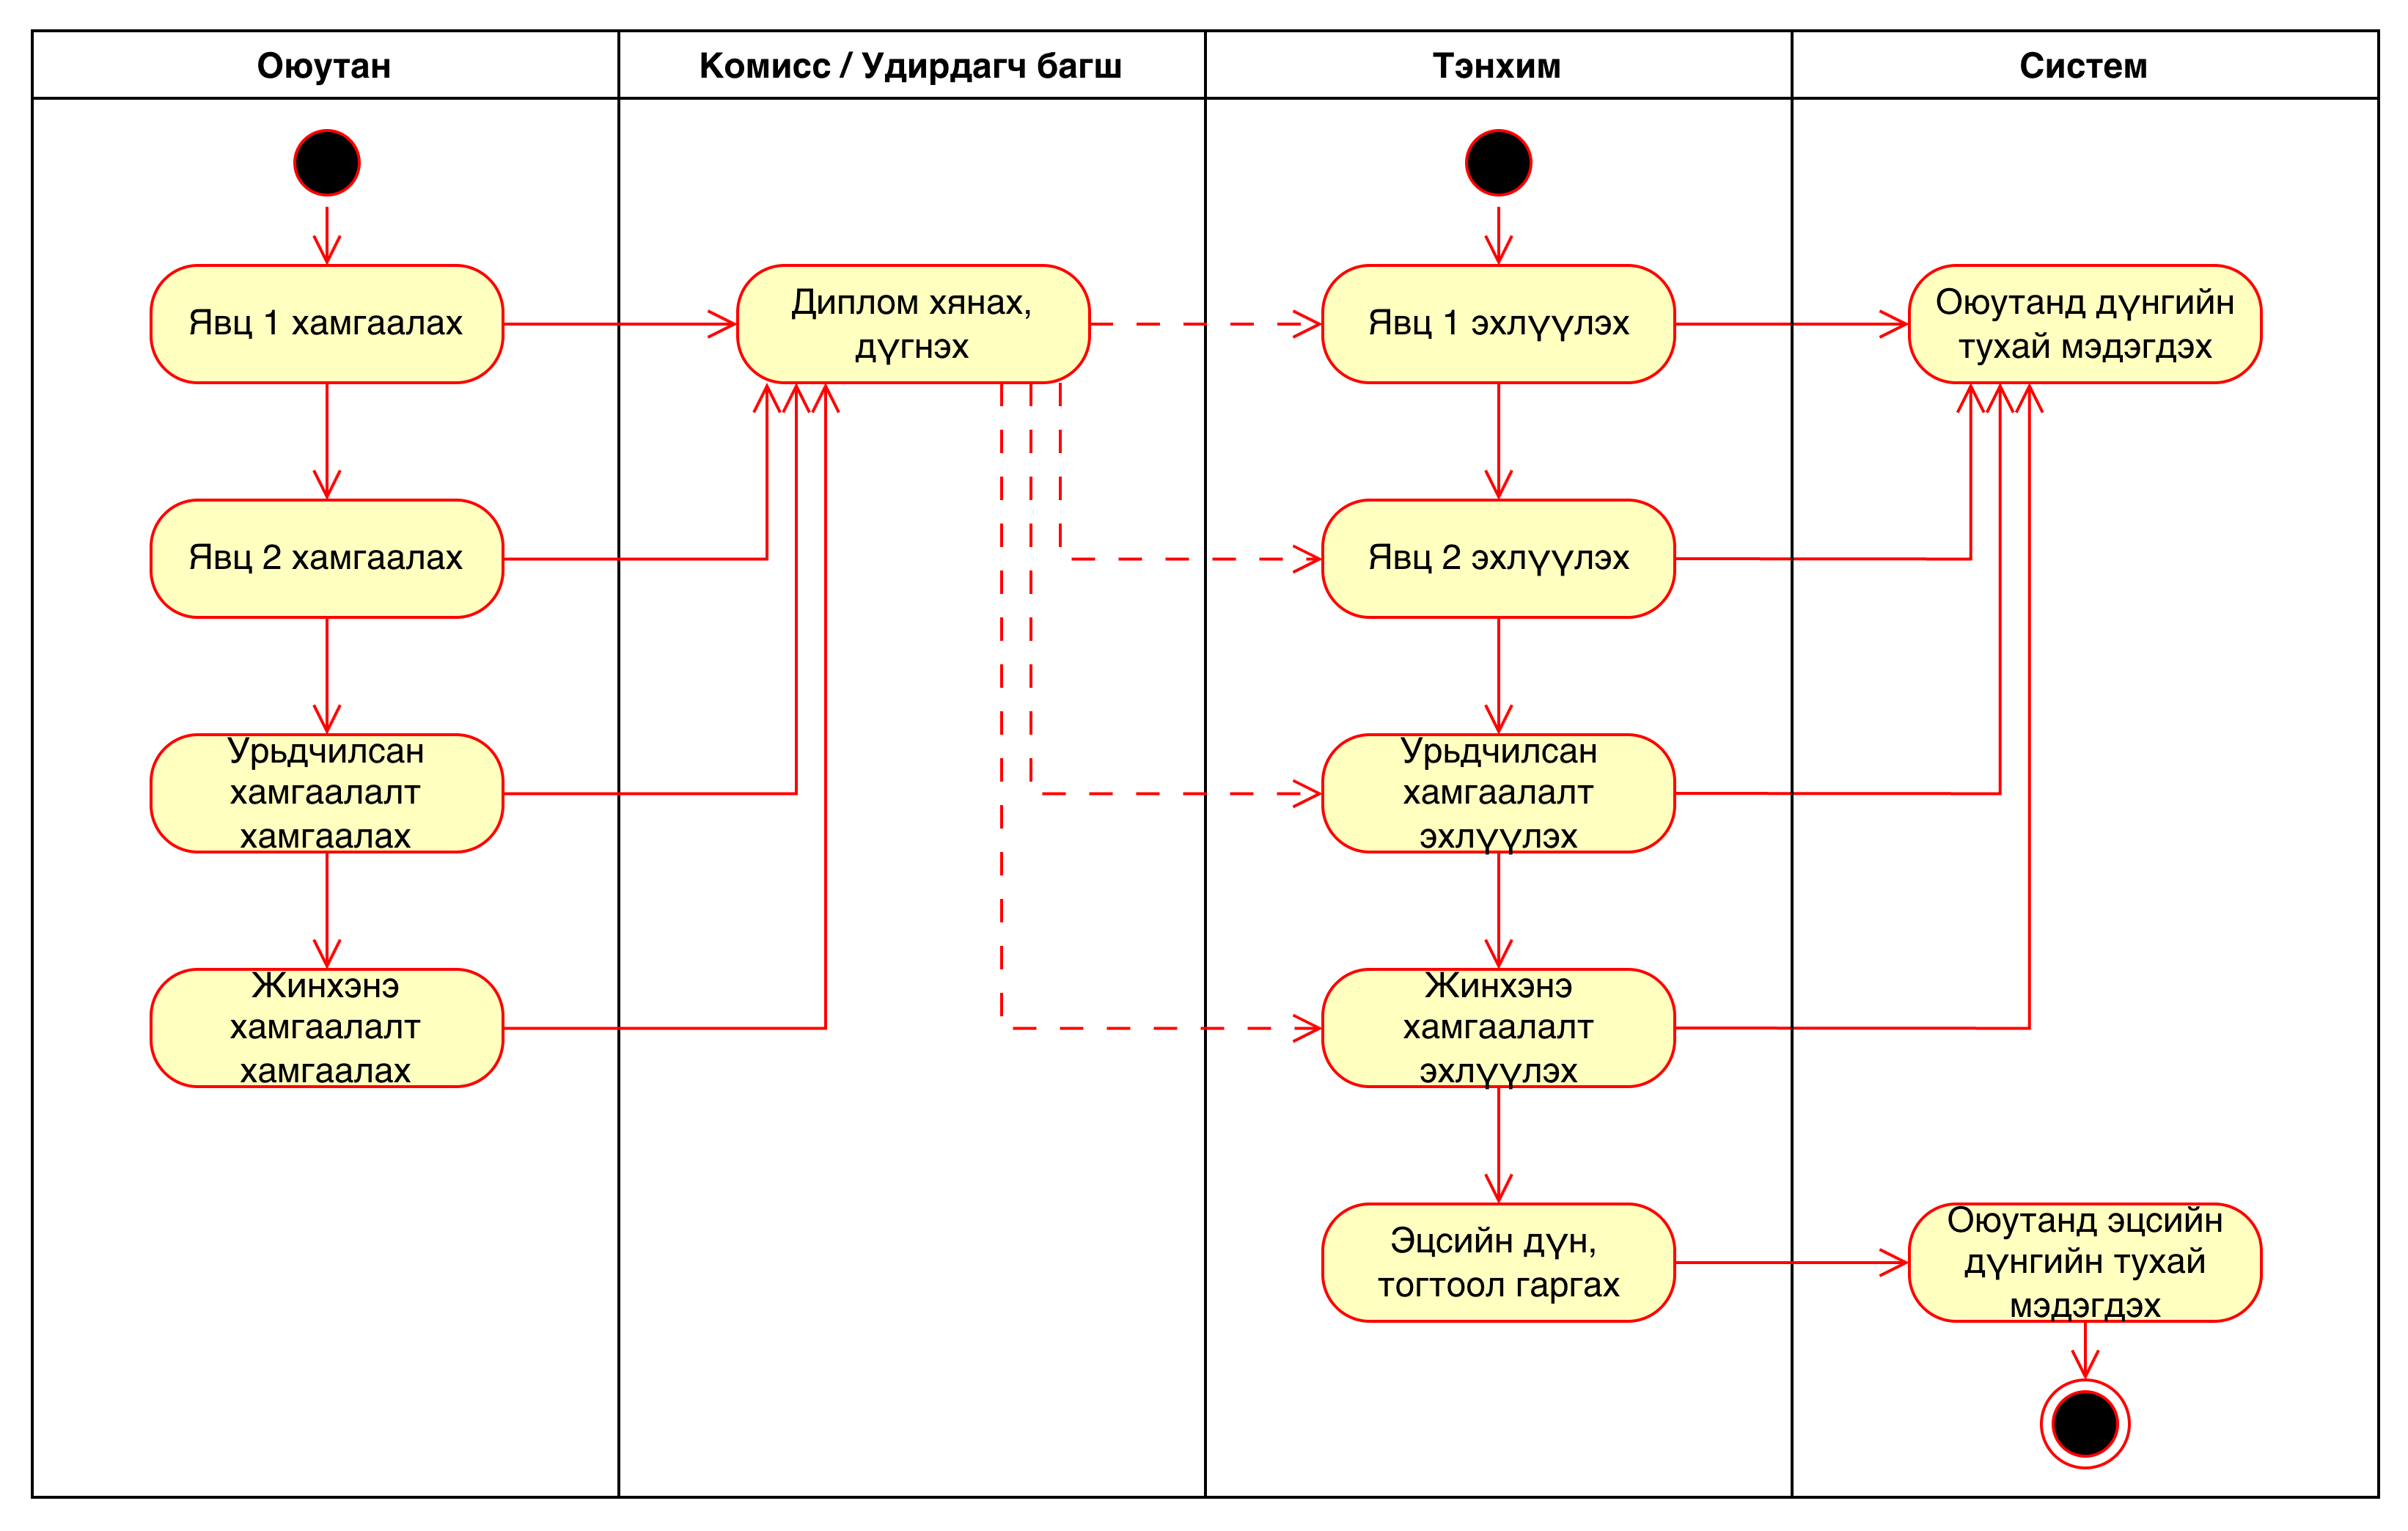
\includegraphics[width=16cm]{images/evaluate.png}
  \caption{БСА-ыг хамгаалах, дүгнэх процесс}
  \label{fig:evaluate}
\end{figure}

\section{Динамик загвар}
\hspace*{1cm} МУИС-ийн Дипломын ажлын удирдлагын системийн динамик загварыг зураг \ref{fig:usecase}-т харуулав. Динамик загварт оюутан, багш, тэнхим, гадны мэргэжилтэн гэсэн тоглогчид оролцох бөгөөд тоглогч тус бүрийн ажлын явцын задаргааг дүрслэв.

\begin{figure}[H]
  \centering
  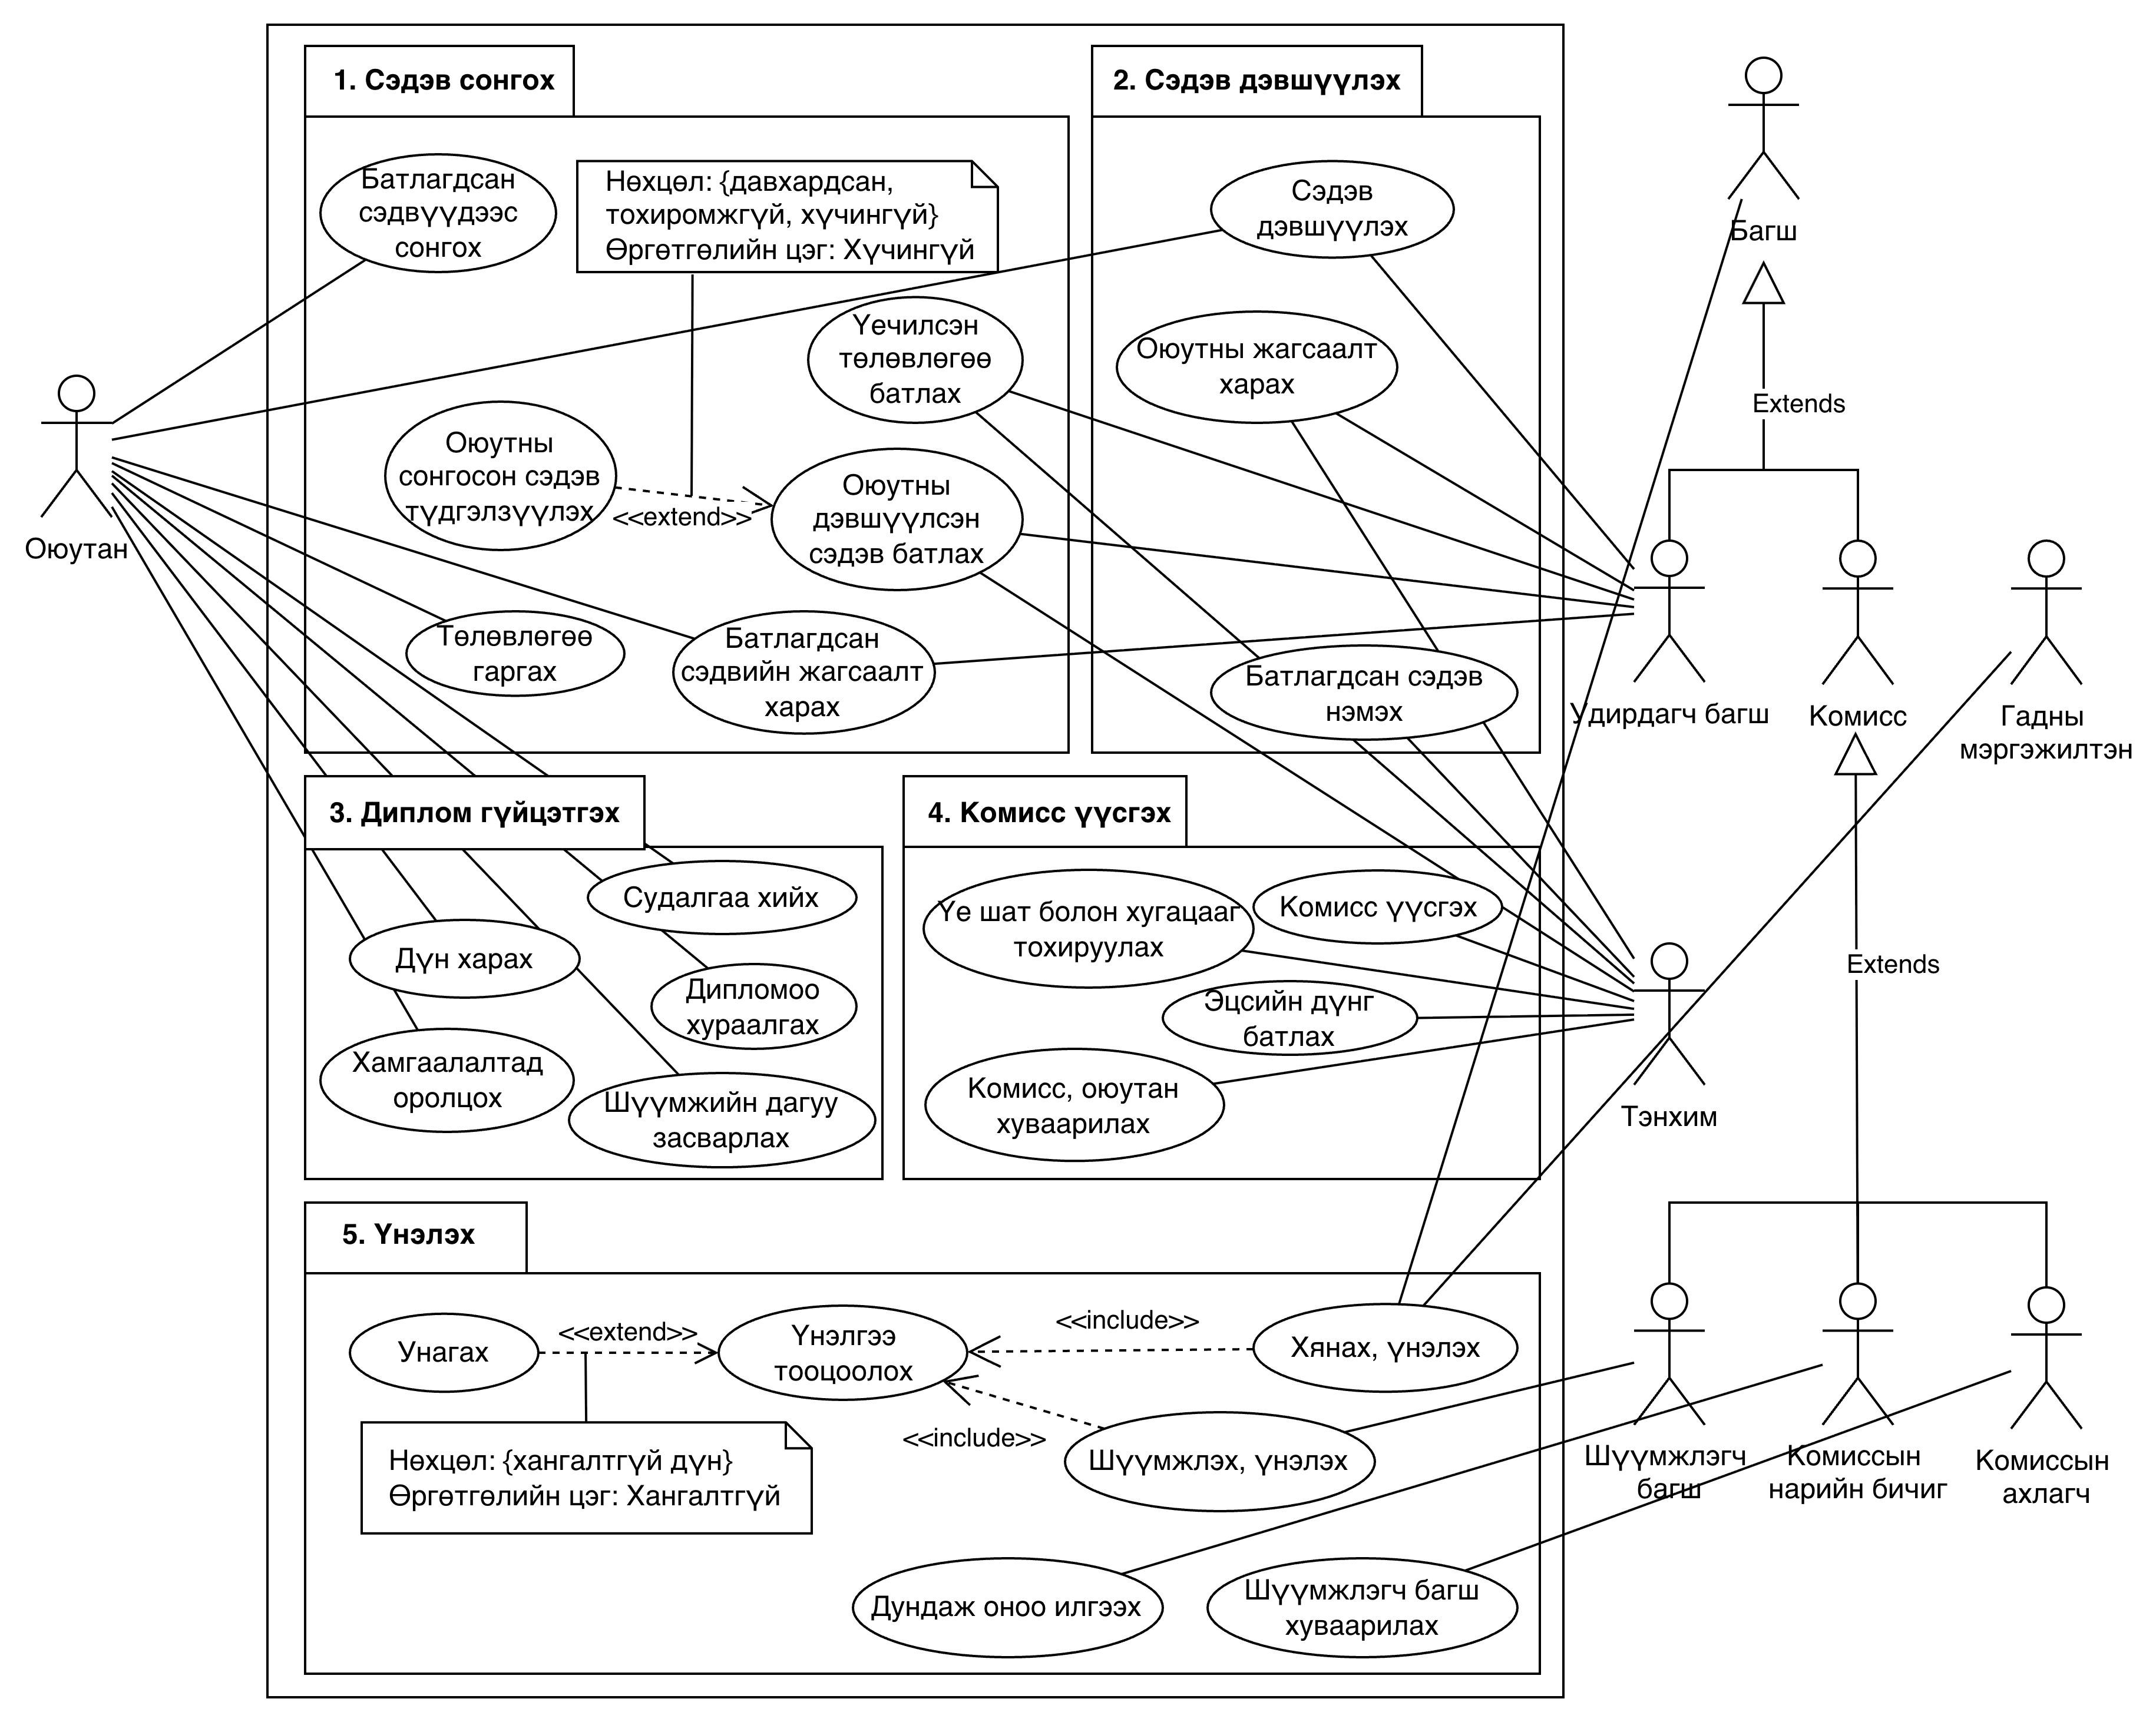
\includegraphics[width=17cm]{images/usecase.png}
  \caption{Дипломын ажлын удирдлагын системийн динамик загвар}
  \label{fig:usecase}
\end{figure}

\begin{table}[H]
\centering
\caption{Дипломын ажлын удирдлагын системийн ажлын явцын тайлбар}
\label{tab:usecase_detail}
\renewcommand{\arraystretch}{0.7}
\begin{tabular}{lcc}
\toprule
\textbf{Ажлын явц} & \textbf{Тоглогч} & \textbf{Тайлбар} \\
\midrule

Батлагдсан сэдвүүдээс сонгох & Оюутан &  \\ 
Батлагдсан сэдвийн жагсаалт харах & Оюутан &  \\ 
Төлөвлөгөө гаргах & Оюутан &   \\
Сэдэв дэвшүүлэх & Оюутан &   \\
Судалгаа хийх & Оюутан &  \\ 
Дипломоо хураалгах & Оюутан &  \\ 
Хамгаалалтад оролцох & Оюутан &  \\ 
Шүүмжийн дагуу засварлах & Оюутан &  \\ 
Дүн харах & Оюутан &  \\ 

Оюутны жагсаалт харах & Тэнхим &  \\ 
Батлагдсан сэдэв нэмэх & Тэнхим &  \\ 
Үечилсэн төлөвлөгөө батлах & Тэнхим &  \\ 
Оюутны дэвшүүлсэн сэдэв батлах & Тэнхим &  \\ 
Комисс үүсгэх & Тэнхим &  \\ 
Үе шат болон хугацааг тохируулах & Тэнхим &  \\ 
Эцсийн дүнг батлах & Тэнхим &  \\ 
Комисс, оюутан хуваарилах & Тэнхим &  \\ 

Сэдэв дэвшүүлэх & Удирдагч багш &  \\ 
Оюутны жагсаалт харах & Удирдагч багш &  \\ 
Үечилсэн төлөвлөгөө батлах & Удирдагч багш &  \\ 
Оюутны дэвшүүлсэн сэдэв батлах & Удирдагч багш &  \\ 
Батлагдсан сэдвийн жагсаалт харах & Удирдагч багш &  \\ 
Хянах, үнэлэх & Удирдагч багш &  \\ 

Шүүмжлэх, үнэлэх & Шүүмжлэгч багш &  \\ 
Хянах, үнэлэх & Шүүмжлэгч багш &  \\ 

Судалгаа хийх & Комиссын нарийн бичиг &  \\ 
Дундаж оноо илгээх & Комиссын нарийн бичиг &  \\ 

Шүүмжлэгч багш хуваарилах & Комиссын ахлагч &  \\ 
Хянах, үнэлэх & Комиссын ахлагч &  \\ 

Хянах, үнэлэх & Гадны мэргэжилтэн &  \\ 

\bottomrule
\end{tabular}
\end{table}